\documentclass{../../../yukibook.cls/yukibook}

\begin{document}

\yukibook{Sistemas Operativos \linebreak en red} 	% Title
  {Rubén Gómez}  % Author
  {2021-2022}    % Year
  {Técnico en Sistemas microinformáticos y redes} % Name of degree
  {\textquote{A very good phrase for a very good book}}	% catch phrase
  {The phrase's author}	% the phrase's author
  {img/cover.png}

%--------------------------------------------------------------------------
% Start your parts, chapters and sections here
%--------------------------------------------------------------------------

%\part{Part 1}

\chapter{Introducción a GNU/Linux}
\section{Un poco de historia}
Para conocer cómo nació el movimiento GNU y el kernel Linux debemos conocer un poco de historia de la informática y cómo evolucionó en los primeros años.

\subsection{El nacimiento de Unix}

\begin{description}
\item[1964-1969]Los laboratorios \textbf{Bell} empiezan un proyecto con el \textbf{MIT} (Instituto Tecnológico de Massachusetts) y \textbf{General Electric} para desarrollar un sistema de \textbf{tiempo compartido} (“time-sharing computing”): se llamaría \textbf{Multics} (Multiplexed Information and Computing Service).

Hasta este momento, los sistemas utilizados eran de un único proceso, la CPU no era compartida por múltiples procesos sino que se ejecutaba por lotes (se les mandaba los procesos a ejecutar y se ejecutaban en orden).

Multics obtuvo licencia libre en el 2007. En Diciembre del 2016 salió la última versión 12.6f.

\itemimage{1969}{r}{0.33}
  {img/Ken_Thompson_and_Dennis_Ritchie--1973.jpg}
  {\href{https://en.wikipedia.org/wiki/Ken_Thompson}{Ken y Dennis . Origen: Wikipedia}}
  {
  Uno de los desarrolladores de Multics, \href{https://en.wikipedia.org/wiki/Ken_Thompson}{Ken Thompson}, decidió escribir su propio sistema operativo. Ken Thompson es conocido también por crear el lenguaje de programación \textbf{B}, el sistema de codificación de caracteres UTF-8 y el lenguaje de programación Go, entre otras cosas.

A Ken Thompson se le une \href{https://en.wikipedia.org/wiki/Dennis_Ritchie}{Dennis Ritchie} y otros, y empiezan a programar un sistema de ficheros jerárquico, el concepto de procesos de computación, ficheros de dispositivos, un intérprete de comandos, … El resultado de lo programado era más pequeño y simple que Multics, lo que se convertiría en Unix. En Agosto ya tendrían el sistema operativo, se auto-gestiona,  tenía un assembler, un editor y una shell de comandos.

Dennis Ritchie es conocido también por crear junto con Ken el lenguaje de programación \textbf{C} (aparece por primera vez en 1972).
}


\item[1970]En ese momento el nuevo sistema operativo se llamaba \textbf{Unics} (\textit{Uniplexed Information and Computing Service}, un juego de palabras en contraposición a  Multics). No tenían todavía dinero de la organización en el desarrollo (era desarrollado por los programadores) y tampoco era multitarea todavía.

A finales de año el sistema ya era conocido como \textbf{UNIX}, y se había portado a la máquina PDP-11.

\textbf{Las primeras versiones de Unix incluían el código fuente} para que las universidades lo pudiesen modificar y así poder extenderlo a sus necesida des.


\item[1971]El sistema se empieza a hacer complejo y como querían que más usuarios lo usasen, crean el sistema de manuales que es utilizado hoy en día (mediante el comando \textbf{"man"}).

\begin{center}
  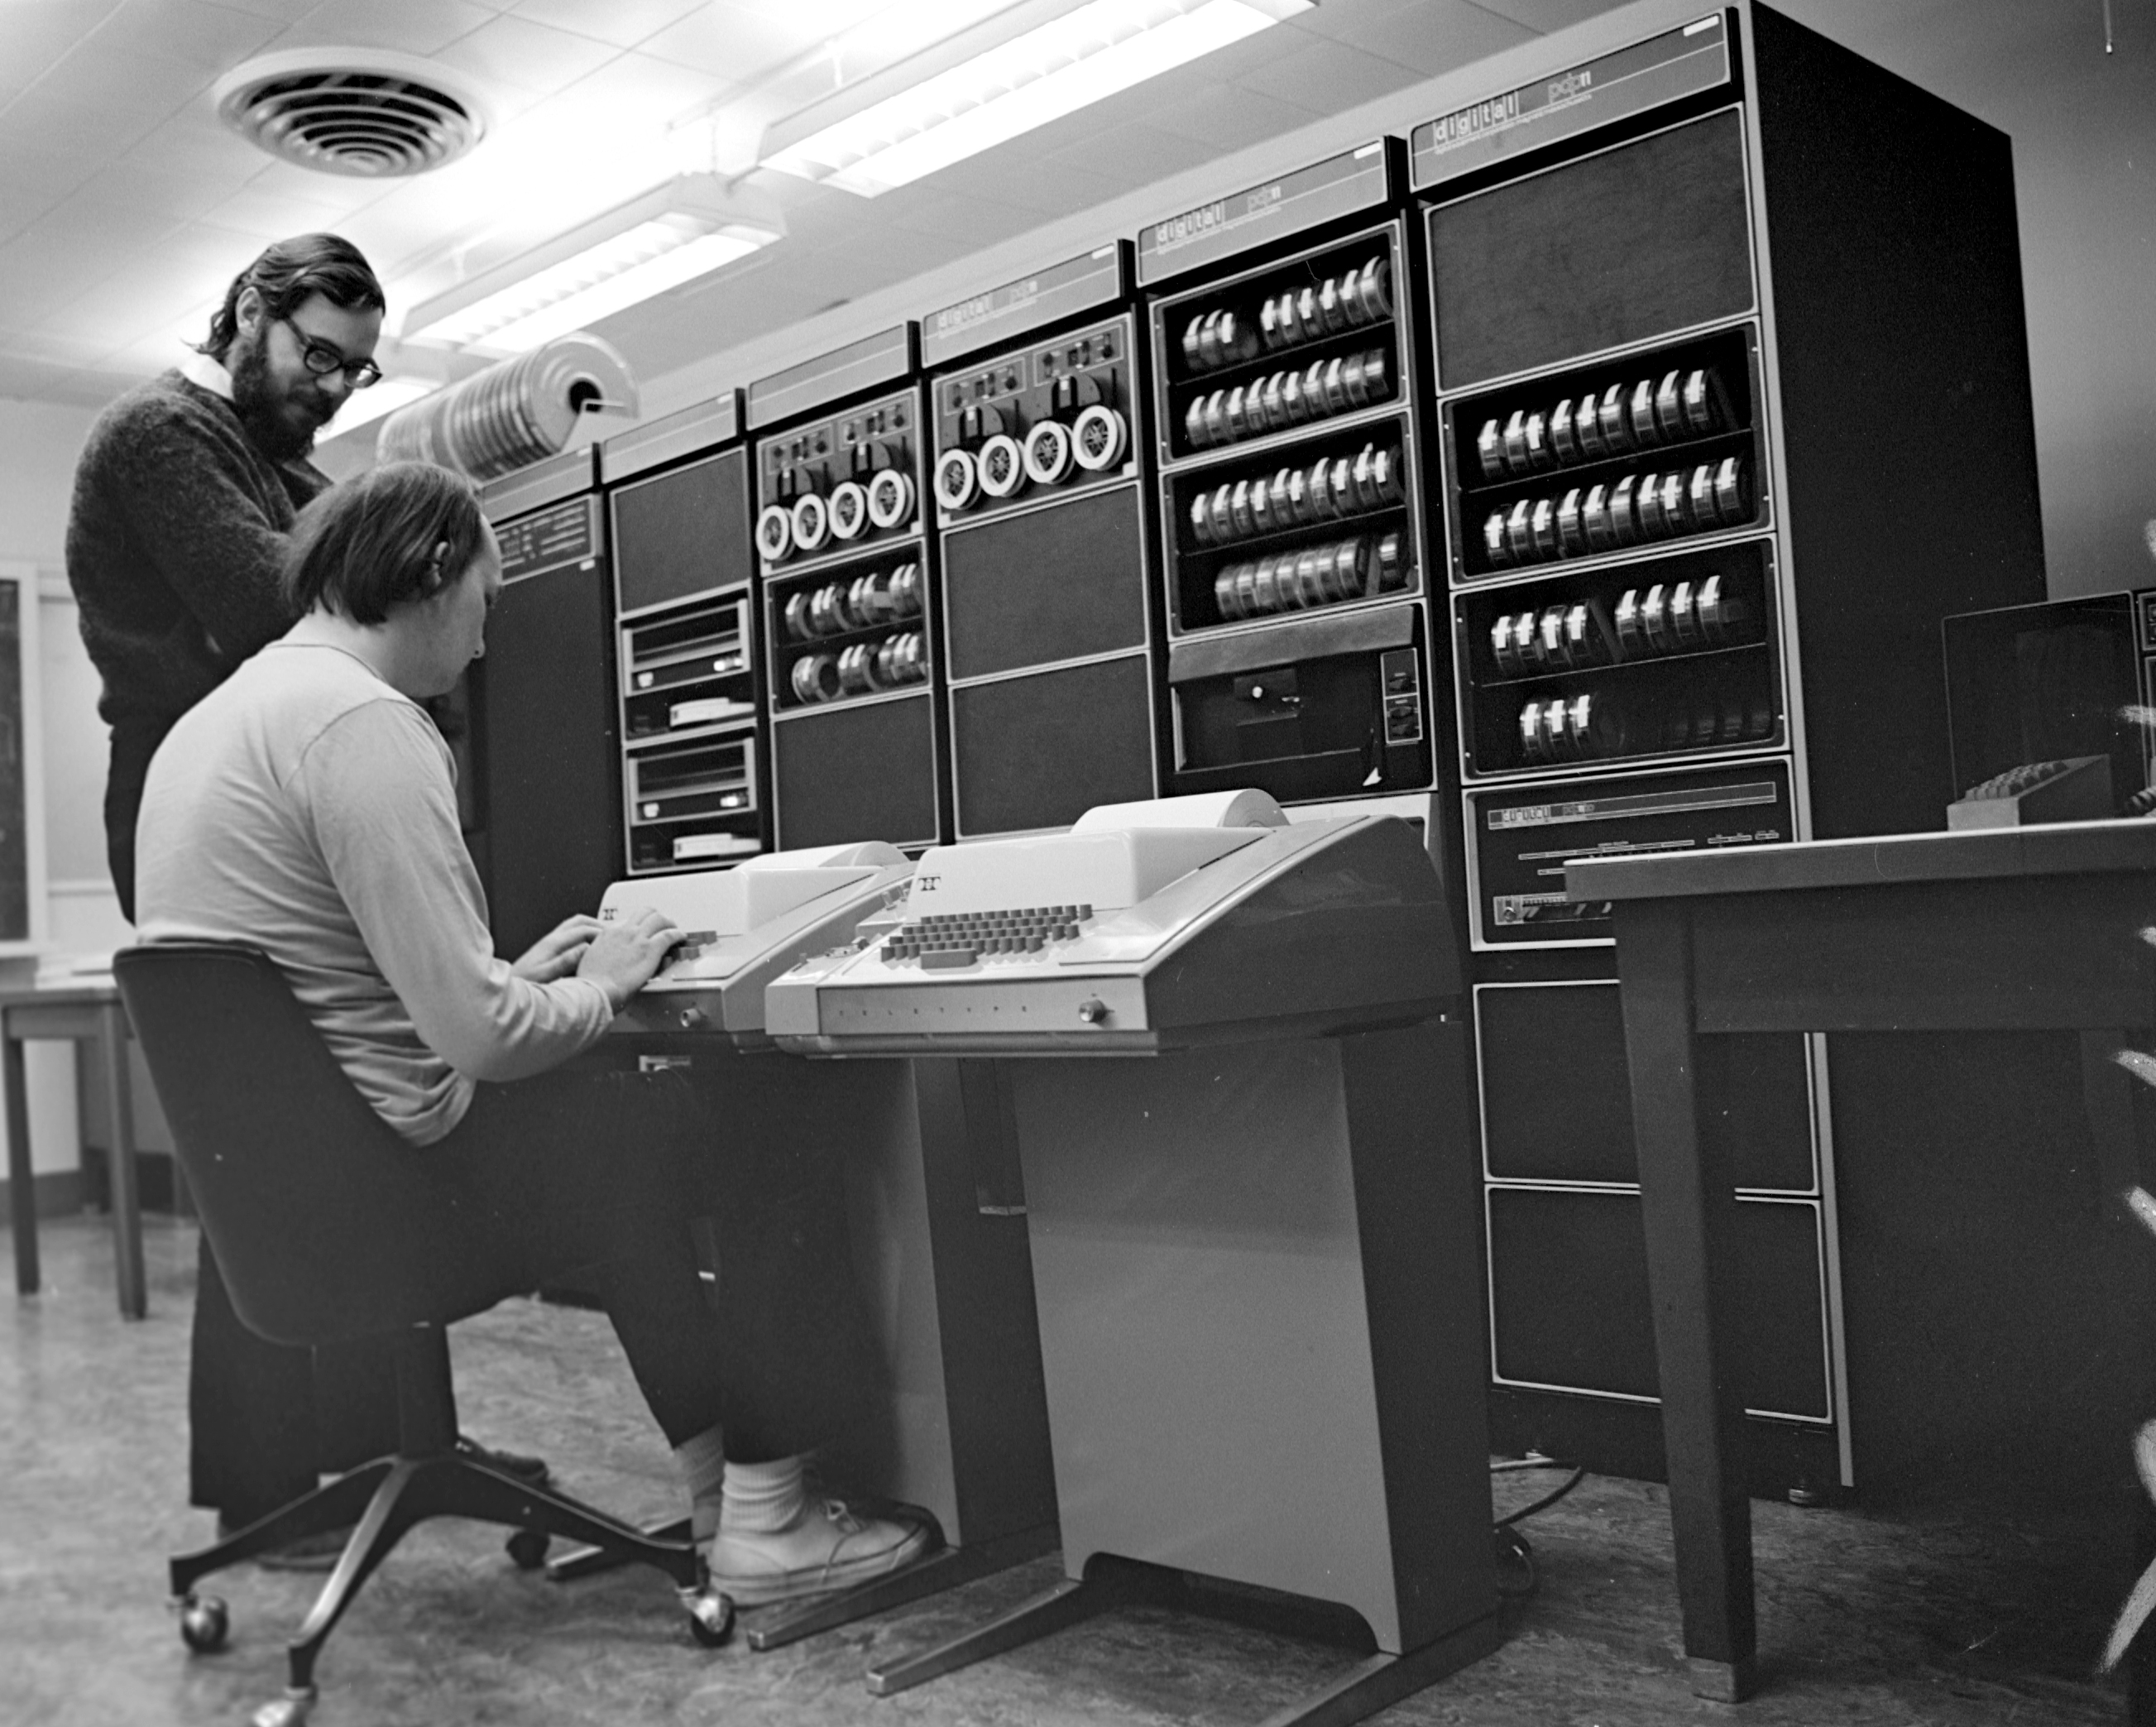
\includegraphics[width=0.8\linewidth]{img/Ken_Thompson_(sitting)_and_Dennis_Ritchie_at_PDP-11_(2876612463).jpg}
  \vspace{-10pt}\captionof{figure}{\href{https://en.wikipedia.org/wiki/Ken_Thompson}{Dennis Ritchie y Ken Thompson. Origen: Wikipedia}}\vspace{-13pt}
\end{center}


\item[1973]La versión 4 del sistema es reescrita completamente en C. Hasta este momento el sistema había estado escrito en ensamblador, por lo que no era portable entre distintos tipos de máquinas, aunque la primera versión portada a otra plataforma fue en 1978. Se cree que había “más de 20” instalaciones del sistema.

\item[1974]La versión 5 se licencia para ser utilizada en \textbf{instituciones educativas}.

\item[1975]La versión 6 se licencia para poder ser utilizadas por empresas por \$20.000 de la época.

\item[1977]La universidad de Berkeley lanza su primera versión de Unix bajo la Berkeley Software Distribution (BSD).

\item[1979]Con la salida de Unix v7, se comienza a portar a los distintos ``microordenadores'' de la época y a los distintos microprocesadores (Motorola 68000, Intel 8086, … ).

\item[1980]Microsoft anuncia su primer Unix para microcomputadoras de 16 bits (Xenix).
\end{description}

\subsection{El nacimiento de GNU (GNU's Not Unix}
\begin{description}

\item[1971]\href{https://en.wikipedia.org/wiki/Richard_Stallman}{Richard Stallman} comienza su carrera en el MIT en el laboratorio de inteligencia artificial.

Es conocido no sólo por el movimiento GNU, si no también por crear GCC y Emacs entre otra gran cantidad de software.

En esa época el software se distribuía de manera abierta para poder ser modificado. Lo habitual era realizar modificaciones para mejorar el software y distribuirlo entre compañeros y universidades.

\itemimage{1982}{r}{0.25}
  {img/Richard_Stallman_2016_Talk_in_Madrid_06.jpg}
  {\href{https://commons.wikimedia.org/wiki/File:Richard_Stallman_2016_Talk_in_Madrid_06.jpg}{Richard Stallman: Wikimedia}}
  {
Richard Stallman quiere modificar el firmware de unas impresoras y el fabricante le pide que firme un acuerdo de no divulgación si le enseñan el código. Esto hace que Stallman se enfurezca y es cuando decide que la situación actual debe cambiar y volver al sistema de intercambio de software anterior.

\item[1983] Se anuncia el nacimiento del proyecto \textbf{GNU}, cuya finalidad es la de construir un sistema operativo completamente libre, compatible con Unix. La idea es dar a los usuarios la libertad y el control de sus ordenadores.

\item[1985] Se lanza el \href{https://www.gnu.org/gnu/manifesto.es.html}{manifiesto GNU}, y ya cuenta con un editor de texto (Emacs), compilador de C, una shell, varias utilidades … El núcleo inicial todavía no es funcional.
}


\item[1986]
Richard Stallman escribe y publica la definición de lo que es Free Software (Software Libre) a través de la \href{https://es.wikipedia.org/wiki/Free_Software_Foundation}{Free Software Foundation}.

\begin{tcolorbox}[title=Aclarando la palabra ``free'':]
\center
\textbf{The word ``free'' in our name does not refer to price; it refers to freedom.}

La palabra ``free'' no se refiere a gratis, si no que se refiere a libertad.
\end{tcolorbox}

Más adelante veremos a qué se refiere sobre libertad en el software.

\end{description}

\subsection{El nacimiento de Minix}
\begin{description}
\item[1987]Andrew S. Tanenbaum crea  Minix como propósito educativo y para enseñar cómo funciona un sistema operativo.

\item[1991]Sale la versión 1.5 de Minix y es portada a distintas arquitecturas (IBM, Motorola 68000, Amiga, Apple Macintosh, …).

\item[1992]Debate con Linus Torvalds sobre la arquitectura del kernel Linux (núcleo monolítico) en lugar de usar un micronúcleo.

\end{description}


\subsection{El nacimiento de Linux}
\begin{description}

\item[1991] Un estudiante en la universidad de Helsinki, \href{https://en.wikipedia.org/wiki/Linus_Torvalds}{Linus Torvalds}, comienza un proyecto personal escrito para su nuevo ordenador, un PC con procesador 80386.

El desarrollo comienza bajo \textbf{Minix}, usando el compilador \textbf{GCC} del movimiento GNU (GCC = GNU Compiler Collection).

El proyecto termina convirtiéndose en un kernel de un sistema operativo y escribió al grupo de noticias de Minix diciendo:

\begin{tcolorbox}[title=Email de Linus Torvalds presentando Linux,sidebyside,righthand width=0.30\linewidth]
  “Hola a todos los que estáis ahí fuera usando minix.\\


  Estoy haciendo un sistema operativo (libre), (solamente por aficion, no será grande ni profesional como el GNU) para clones 386(486) AT.

  ...

  PD. Sí – está libre de cualquier código de minix, y tiene un sistema de ficheros multi-hilo. NO es portable (usa el cambio de tareas del 386 etc), y probablemente nunca soporte otra cosa que no sean los discos duros AT, porque es todo lo que tengo :-(. ”
  \tcblower
  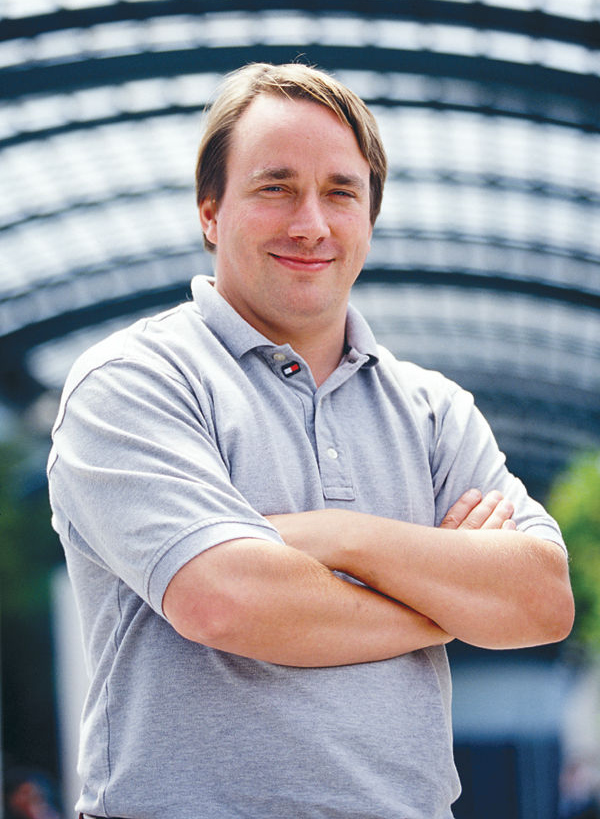
\includegraphics[width=\linewidth]{img/Linus_Torvalds.jpeg}
  \vspace{-30pt}\captionof{figure}{\href{https://en.wikipedia.org/wiki/Linus_Torvalds}{Linus torvalds. Origen: Wikipedia}}
\end{tcolorbox}


\item[1992] Originalmente la licencia de Linux era propia e impedía el uso comercial de Linux. En la versión 0.99 esto cambia y se cambia a la licencia GNU Public License (\textbf{GPL}).

\item[1993] El proyecto cuenta con más de 100 desarrolladores. El kernel se adapta al entorno del proyecto GNU. Nace la distribución \textbf{Debian} (una de las más importantes a día de hoy)

\begin{center}
  
\includegraphics[width=0.5\linewidth]{img/debian-logo.jpg}
  \vspace{-10pt}\captionof{figure}{\href{https://www.debian.org}{Debian}}
\end{center}

\item[1994] Se libera la versión 1.0. El proyecto XFree86 se une y Linux consigue interfaz gráfico. Nacen las primeras distribuciones comerciales \textbf{Red Hat} y \textbf{Suse}.

\item[1998] Empresas como \textbf{IBM}, \textbf{Compaq} y \textbf{Oracle} anuncian que apoyan a Linux. Nace el interfaz gráfico \textbf{KDE}.

\item[1999] Nace el interfaz gráfico \textbf{GNOME} como reemplazo a KDE, ya que KDE hacía uso de una librería propietaria en aquel momento (QT).

\item[2001] Steve Ballmer (CEO de Microsoft) dice: \textbf{“Linux es un cáncer”}.

\item[2002] Se libera OpenOffice (originalmente suite ofimática de Sun Microsystems). Nace Mozilla (hoy día:  Firefox).

\item[2003] IBM lanza un anuncio para la Linux Foundation: \href{https://www.youtube.com/watch?v=x7ozaFbqg00}{https://www.youtube.com/watch?v=x7ozaFbqg00}

\item[2004] Nace \textbf{Ubuntu} (basándose en Debian) y Steve Ballmer (CEO de Microsoft) dice que Linux infringe muchas de sus patentes.

\item[2008] Nace \textbf{\href{https://es.wikipedia.org/wiki/Android}{Android}}, sistema operativo con kernel Linux. Actualmente es el sistema operativo de móviles que más terminales tiene.

\item[2009] Red Hat iguala a Sun Microsystem en capitalización bursátil (un gran logro simbólico).

\item[2014] Satya Nadella (CEO de Microsoft) muestra en una presentación la siguiente transparencia:

\begin{center}
  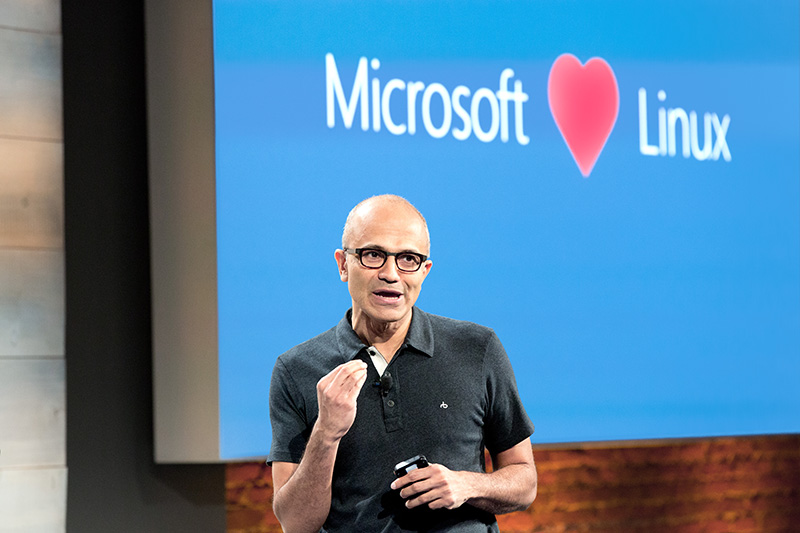
\includegraphics[width=0.5\linewidth]{img/Microsoft_Linux.jpg}
  \vspace{-10pt}\captionof{figure}{\href{https://commons.wikimedia.org/wiki/File:Microsoft_Linux.jpg}{Origen: Wikipedia}}
\end{center}


\item[2016]
Microsoft anuncia \href{https://es.wikipedia.org/wiki/Windows_Subsystem_for_Linux}{WSL} (\textit{Windows Subsystem for Linux}) y se puede instalar en Windows 10 y Windows Server 2019. Permite correr ejecutables de Linux nativamente.

\end{description}

\subsection{Cronograma de sistemas Unix}
En el siguiente cronograma se puede ver la línea temporal de los sistemas Unix:

\begin{center}
  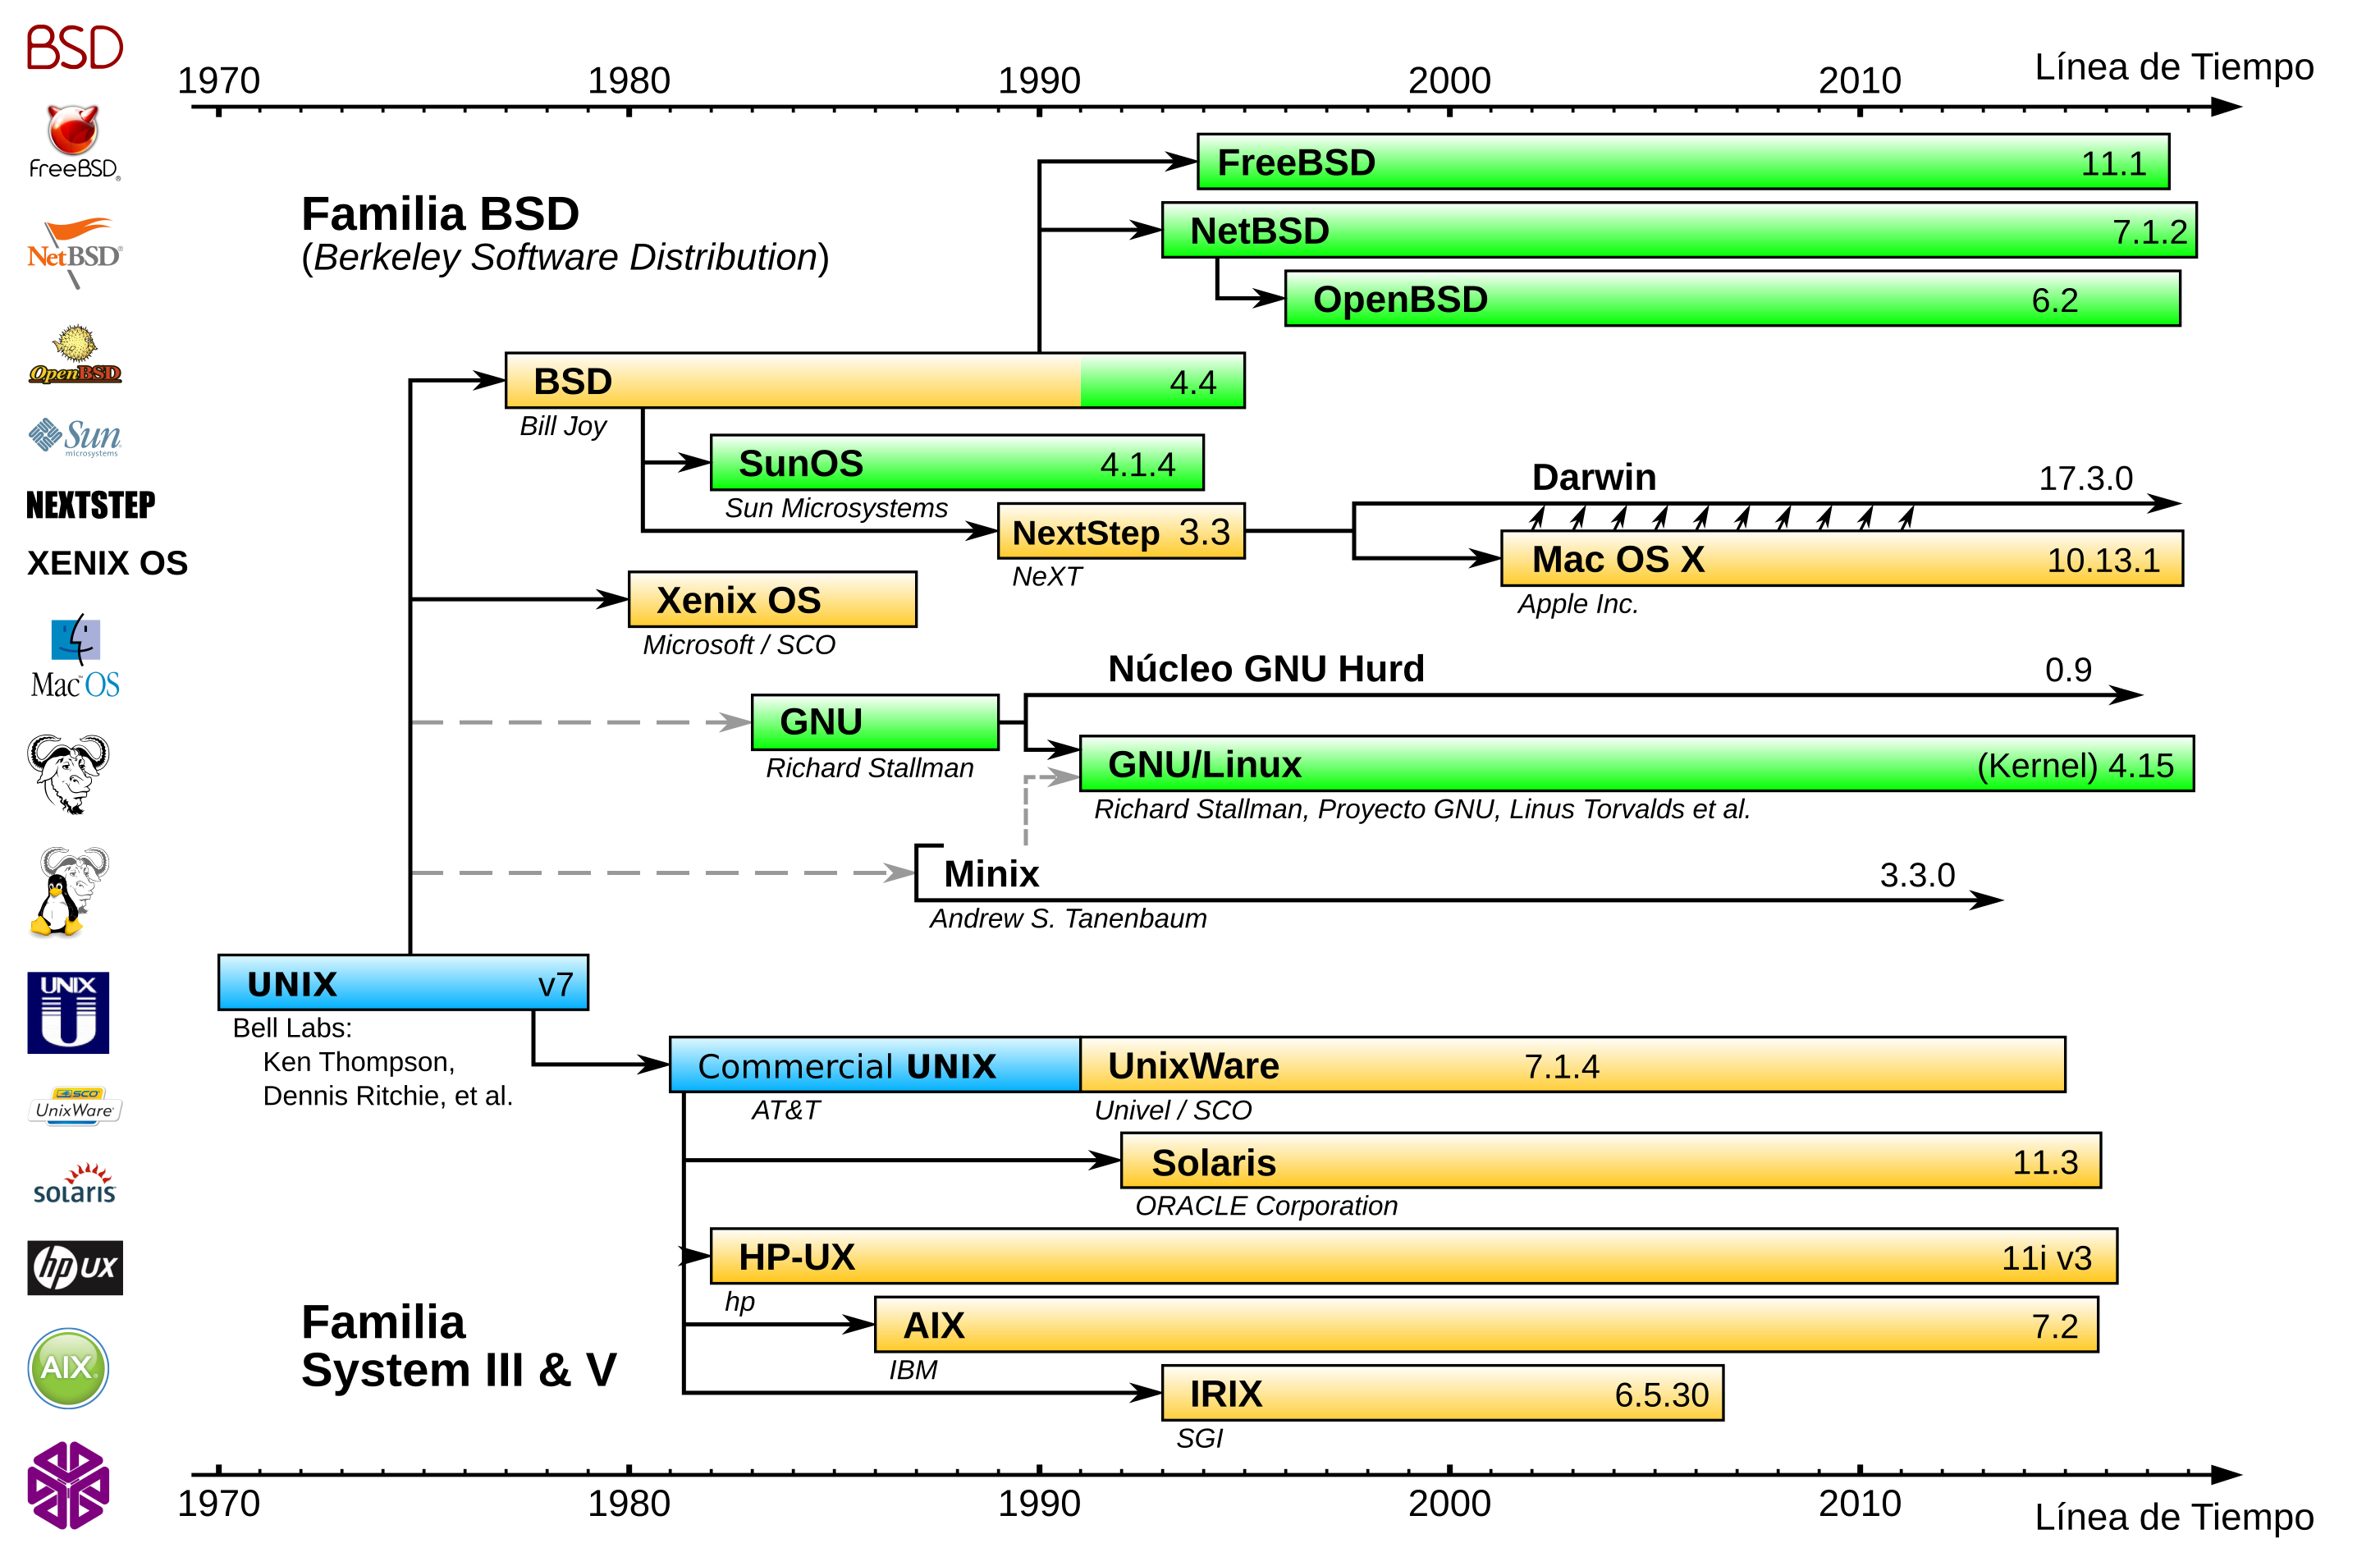
\includegraphics[width=0.7\linewidth]{img/Evolución_UNIX.png}
  \vspace{-10pt}\captionof{figure}{\href{https://commons.wikimedia.org/wiki/File:Evolución_UNIX.png}{Origen: Wikipedia}}
\end{center}

\section{Resumen}
Linux es conocido como un sistema operativo libre pero el nombre de Linux se  centra única y exclusivamente en el \textbf{kernel} (o \textbf{núcleo}) del sistema operativo.

El sistema operativo completo debería llamarse \textbf{GNU/Linux}, ya que el kernel es una “pequeña” parte (aunque muy importante) dentro de todo el sistema operativo. El resto de herramientas utilizadas en el sistema operativo pertenecen al proyecto GNU.


\chapter{Licencias Libres}
\section{Software Libre}

En 1986 Richard Stallman saca a la luz la definición de lo que es Free Software (Software Libre) a través de la \href{https://es.wikipedia.org/wiki/Free_Software_Foundation}{Free Software Foundation}:

\begin{tcolorbox}[title=Definición de Free Software:]
    \center
    \textbf{The word ``free'' in our name does not refer to price; it refers to freedom.}

    La palabra ``free'' no se refiere a gratis, si no que se refiere a libertad.
\end{tcolorbox}


Las libertad en el software se refiere a:
\begin{tcolorbox}[title=Libertades del Software Libre:]
    \begin{enumerate}
        \setcounter{enumi}{-1}
        \item La libertad de ejecutar el programa, para cualquier propósito .

        \item La libertad de estudiar cómo trabaja el programa, y cambiarlo para que haga lo que usted quiera. El acceso al código fuente es una condición necesaria para ello.

        \item La libertad de redistribuir copias para que pueda ayudar al prójimo.

        \item La libertad de mejorar el programa y publicar sus mejoras, y versiones modificadas en general, para que se beneficie toda la comunidad. El acceso al código fuente es una condición necesaria.
    \end{enumerate}
\end{tcolorbox}

El movimiento del Free Software es un movimiento que tiene que ver más con la filosofía y la ética que con la tecnología en sí misma.


\subsection{Copyleft y GNU Public License (GPL)}
Es una práctica legal que consiste en el ejercicio del derecho de autor (copyright en inglés) con el objetivo de propiciar el libre uso y distribución de una obra, exigiendo que los concesionarios preserven las mismas libertades al distribuir sus copias y derivados (\href{https://es.wikipedia.org/wiki/Copyleft}{Wikipedia}).

\begin{center}
  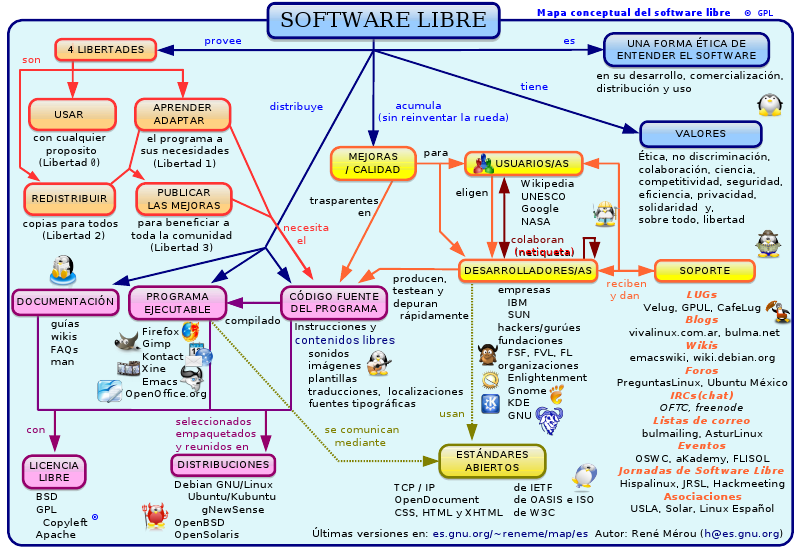
\includegraphics[width=\linewidth]{img/Mapa_conceptual_del_software_libre.png}
  \vspace{-30pt}\captionof{figure}{\href{https://commons.wikimedia.org/wiki/File:Mapa_conceptual_del_software_libre.png}{Mapa conceptual del Software Libre: Wikipedia}}\vspace{-20pt}
\end{center}

Con esto nació la licencia GNU GPL, la cual permite al usuario final la libertad de usar, estudiar, compartir y modificar el software recibido. Tiene que quedar claro que un programa comercial puede ser Software Libre.

\subsection{Diferencias con el Open Source}
Los programas Open Source son aquellos que podemos ver el código fuente pero esto no quiere decir que podamos modificarlo o adaptarlo a nuestras necesidades.

El Open Source es menos restrictivo que el Software Libre y se puede decir que todo Software Libre es Open Source, pero no todo Open Source tiene por qué ser libre.


\section{Licencias libres más conocidas}
Un listado de las licencias libres más utilizadas:

\begin{itemize}
    \item \href{https://es.wikipedia.org/wiki/GNU_General_Public_License}{GNU GPL}
    \item \href{https://es.wikipedia.org/wiki/Licencia_BSD}{BSD}
    \item \href{https://es.wikipedia.org/wiki/Licencia_MIT}{MIT}
    \item \href{https://es.wikipedia.org/wiki/Apache_License}{Licencia Apache}
    \item \href{https://es.wikipedia.org/wiki/Licencia_PHP}{Licencia PHP}
    \item \href{https://es.wikipedia.org/wiki/Licencias_Creative_Commons}{Creative Commons} (no todas las versiones). Más utilizadas en contenido multimedia.
\end{itemize}


\chapter{Sistema de ficheros en GNU/Linux}
El sistema de ficheros en GNU/Linux, al igual que en Unix, es jerárquico, comenzando en la raíz denominada “/”. Partiendo de esta raíz, el resto del sistema de ficheros nace en forma de ramificaciones generando lo que se denominan “rutas de ficheros”, que es el camino completo para llegar al mismo.

\section{Filesystem Hierarchy Standard}
Debido a que en GNU/Linux todo se representa como ficheros (discos, dispositivos, programas, … ) es necesario que exista un orden a la hora de ser almacenados. Con esa intención nace en 1993 el estándar de la jerarquía de ficheros de Linux, enfocado a reestructurar los archivos. Posteriormente se unieron otros derivados de UNIX (la comunidad de desarrollo de BSD) por lo que terminó adoptando el nombre FHS.

Aún siendo un estándar, no todas las distribuciones lo siguen al pie de la letra, y otros Unix, como MacOS, tienen sus propias rutas especiales.


\section{Directorios importantes}
A continuación se exponen los directorios más importantes del sistema junto con la descripción del contenido que deben de tener:
\begin{itemize}

    \item \textbf{/boot/}: archivos de arranque del kernel, normalmente junto con la configuración utilizada para compilarlos.
    \item \textbf{/dev/}: contiene archivos especiales de bloque que representan los dispositivos del hardware que está corriendo el sistema operativo
    \item \textbf{/etc/}: contiene los archivos de configuración del servidor y de los servicios que corren en él. Está subdividido en directorios por servicios o configuraciones.
    \item \textbf{/home/}: los directorios de trabajo de los usuarios normales del sistema
    \item \textbf{/lib/}: librerías que hacen funcionar a los programas
    \item \textbf{/root/}: es la home del usuario root
    \item \textbf{/var/}: archivos variables del sistema
    \begin{itemize}
      \item \textbf{/var/lib/}: aquí se suelen guardar los ficheros de los programas que “crecen”: bases de datos, ficheros caché…
      \item \textbf{/var/log/}: los logs del sistema
    \end{itemize}
\end{itemize}

Junto a todos estos directorios, se ha separado los lugares en los que van los binarios, o ejecutables de los programas. Lo habitual es que se encuentren en estas rutas:

\begin{itemize}
    \item \textbf{/bin/}: aplicaciones esenciales del sistema
    \item \textbf{/sbin/}: aplicaciones que en principio sólo debería ejecutar el usuario root o programas de administración del sistema
    \item \textbf{/usr/bin/}: ejecutables de usuario
    \item \textbf{/usr/sbin/}: ejecutables de superusuario
\end{itemize}
Aunque las rutas de los ejecutables denotan quién debería ejecutar el programa, en la vida real no tiene por qué ser una limitación.

\section{Dispositivos de almacenamiento y discos duros}
En sistemas operativos Windows es habitual que cada partición cuente con una letra para acceder a ella, al igual que ocurre cuando introducimos un dispositivo de almacenamiento externo (un pendrive).

Tal como se ha comentado, en sistemas Unix el sistema de ficheros es una jerarquía, y por tanto todo dispositivo de almacenamiento nuevo deberá estar montado bajo la raíz “/”. Hoy día, en distribuciones con escritorio, al introducir un pendrive éste es auto-montado (es accesible) desde la ruta \textbf{/media/}, donde aparecerán tantos directorios como discos hayamos conectado.

\subsection{Almacenamiento permanente}
Si queremos que un disco duro nuevo sea permanente en nuestro sistema, podremos montarlo en cualquier lugar de la estructura jerárquica. Debido a este sistema, el usuario final no se tendrá que preocupar en almacenar los ficheros en una ruta distinta, si no que será el administrador el que haya hecho que esa ruta ahora pertenezca a un disco duro nuevo.

Imaginemos que el sistema operativo se ha instalado en un disco duro pequeño de 32Gb de espacio y se está llenando, y el directorio que más ocupa es el directorio de los usuarios. Podremos añadir al servidor un nuevo disco duro montado en /home y por tanto a partir de ahora los datos guardados en /home estarán en un nuevo disco duro más grande.

\begin{mycode}{Ejemplo de discos en un sistema con ``lsblk''`}{console}{}
root@vega:~# lsblk
NAME                       MAJ:MIN RM   SIZE RO TYPE MOUNTPOINTS
sda                          8:0    0   1,8T  0 disk
└─sda1                       8:1    0   1,8T  0 part /home/backup

sdb                          8:16   0   3,6T  0 disk
└─sdb1                       8:17   0   3,6T  0 part /home/disco4tb
sdc                          8:32   0 447,1G  0 disk
├─sdc1                       8:33   0   529M  0 part
├─sdc2                       8:34   0   100M  0 part
├─sdc3                       8:35   0    16M  0 part
└─sdc4                       8:36   0 446,5G  0 part
nvme0n1                    259:0    0 931,5G  0 disk
├─nvme0n1p1                259:1    0   512M  0 part
└─nvme0n1p2                259:2    0   800G  0 part /home
nvme1n1                    259:3    0 931,5G  0 disk
├─nvme1n1p1                259:4    0   512M  0 part /boot/efi
├─nvme1n1p2                259:5    0    90G  0 part /
├─nvme1n1p3                259:6    0   300G  0 part
│ ├─VMs-ubuntu--20.04--so1 254:0    0    10G  0 lvm
│ ├─VMs-manjaro            254:2    0    20G  0 lvm
│ └─VMs-win10              254:3    0    35G  0 lvm
└─nvme1n1p4                259:7    0 156,2G  0 part
\end{mycode}


\chapter{Gestión de usuarios locales en GNU/Linux}
En las distribuciones GNU/Linux lo habitual suele ser que existan al menos dos usuarios tras una instalación:

\begin{itemize}
    \item \textbf{root}: usuario administrador o súper usuario.
    \item \textbf{usuario no-privilegiado}: durante la instalación de la distribución nos suele preguntar para crear un usuario del sistema, que no tendrá privilegios.
\end{itemize}


El usuario root, como se ha dicho previamente, es el administrador del sistema, tiene permisos para realizar cualquier tarea dentro de nuestro sistema: instalar paquetes, desinstalarlos, modificar cualquier fichero, realizar formateos... Por lo tanto, el \textbf{realizar tareas como usuario root puede ser peligroso si cometemos algún fallo}.

Las buenas prácticas nos dicen que las tareas cotidianas del sistema deberíamos realizarlas como usuario normal y \textbf{sólo convertirnos en root cuando sea estrictamente necesario}.

\section{Creación de usuarios locales}

Tras instalar el sistema, veremos que se nos han creado varios usuarios en el sistema, aparte del usuario \textbf{root} y el usuario \textbf{no-privilegiado}. Para poder ver los usuarios que existen en nuestro sistema podemos verlo en el fichero  \mintinline{console}{ /etc/passwd }  o podríamos obtener un listado ejecutando el siguiente comando:

\begin{mycode}{Listar usuarios del sistema}{console}{}
# cut -d: -f1 /etc/passwd
\end{mycode}

Para crear un usuario:

\begin{mycode}{Crear usuarios del sistema}{console}{\small}
# adduser mikeldi

Añadiendo el usuario `mikeldi' ...
Añadiendo el nuevo grupo `mikeldi' (1001) ...
Añadiendo el nuevo usuario `mikeldi' (1001) con grupo `mikeldi' ...
Creando el directorio personal `/home/mikeldi' ...
Copiando los ficheros desde `/etc/skel' ...
Nueva contraseña:
Vuelva a escribir la nueva contraseña:
passwd: contraseña actualizada correctamente
Cambiando la información de usuario para mikeldi
Introduzca el nuevo valor, o pulse INTRO para usar el valor predeterminado
    Nombre completo []:
    Número de habitación []:
    Teléfono del trabajo []:
    Teléfono de casa []:
    Otro []:
¿Es correcta la información? [S/n]
\end{mycode}

Y la línea que nos creará en el fichero  \mintinline{console}{ /etc/passwd }   es:
\begin{center}
 \mintinline{console}{ mikeldi:x:1001:1001:mikeldi,,,:/home/mikeldi:/bin/bash }
\end{center}

El fichero  \mintinline{console}{ /etc/passwd }  nos muestra los datos de los usuarios, siendo un fichero que tiene distintos datos separados por “:”, siendo cada apartado:

\#\# TODO: TABLA usuario

En las primeras versiones GNU/Linux la contraseña de los usuarios aparecía en el propio fichero /etc/passwd, lo que suponía un problema en la seguridad, ya que no estaban cifradas. Actualmente, las contraseñas de los usuarios se almacenan cifradas en el fichero \mintinline{console}{ /etc/shadow }. El fichero es similar al passwd, estando separados los apartados por “:”

\#\# TODO: tabla SHADOW


En el apartado de la contraseña podemos saber cierta información acerca de la misma ya que tiene el siguiente formato: \textbf{“\$id\$salt\$hashed”}
\begin{itemize}
    \item \textbf{id}: el algoritmo utilizado para cifrar la contraseña
    \begin{itemize}
        \item \$1\$ – MD5
        \item \$2a\$ – Blowfish
        \item \$2y\$ – Eksblowfish
        \item \$5\$ – SHA-256
        \item \$6\$ – SHA-512
    \end{itemize}
\end{itemize}

Aparte, también podemos encontrarnos con:
\begin{itemize}
    \item Contraseña vacía:  Si no hay contraseña, al pedirnos la contraseña a la hora de hacer login será suficiente con pulsar “intro”.
    \item \textbf{!}, \textbf{*}: la cuenta está bloqueada para la contraseña. El usuario no podrá loguearse utilizando la contraseña. Resulta útil si queremos bloquear el acceso con contraseña pero no con otros métodos (clave pública SSH).
    \item \textbf{*LK*}: cuenta bloqueda. El usuario no podrá loguearse.
    \item \textbf{*NP*}, \textbf{!!}: Nunca se ha puesto una contraseña
\end{itemize}


\section{Gestión de grupos}
En algunas distribuciones GNU/Linux, al crear un usuario directamente nos crea un grupo para el nuevo usuario. En otras, el usuario pertenece al grupo “users”.

Para saber los grupos a los que pertenece un usuario podemos ejecutar el comando \mintinline{console}{ groups }. Los grupos del sistema aparecen en el fichero \mintinline{console}{ /etc/group }, y al igual que los ficheros vistos previamente, están separados por “:”.

\#\# TODO: tabla grupos


\section{Permisos de ficheros}
En GNU/Linux los ficheros cuentan con 3 tipos de permisos:
\begin{itemize}
    \item lectura (\textbf{r}ead): el usuario puede leer el fichero
    \item escritura (\textbf{w}rite): el usuario puede escribir en el fichero
    \item ejecución (e\textbf{x}ecute): el usuario puede el fichero o puede ver el contenido de un directorio
\end{itemize}


Todos ello para los distintos usuarios que pueden existir en el sistema:
\begin{itemize}
    \item \textbf{dueño del fichero}: la persona que ha creado el fichero
    \item \textbf{grupo}: los usuarios pertenecientes al grupo al que pertenece el fichero tendrán ciertos privilegios
    \item \textbf{el resto de usuarios}: los permisos que tendrán el resto de usuarios que no son ni el dueño ni pertenecen al grupo
\end{itemize}

Todo ello se puede visualizar en el sistema de ficheros si listamos los permisos del fichero:

\begin{mycode}{Crear usuarios del sistema}{console}{\small}
$ ls -lh fichero.txt
-rw-r--r-- 1 mikeldi mikeldi 0 dic  8 19:17 fichero.txt
\end{mycode}

Los permisos se pueden ver en los primeros 10 caracteres:


\part{Anexos}

\graphicspath{{../../../anexos/instalar_ubuntu_lts/}}
\hypertarget{instalar_ubuntu_lts}{}

\chapter{Instalar Ubuntu 20.04 LTS}
En este anexo realizaremos la instalación de la distribución Ubuntu 20.04 LTS en su versión para servidores. En este anexo no se va a explicar cómo realizar la creación de una máquina virtual donde se aloja el sistema operativo, ya que existen distintos tipos de virtualizadores.

No se realizará una guía “paso a paso”, sino que se centrará en las partes más importantes de la instalación y en las que más dudas puedan surgir.

\section{Descargar Ubuntu 20.04}
La ISO la obtendremos de la \href{https://ubuntu.com/#download}{web oficial} y seleccionaremos la versión 20.04 LTS de Ubuntu Server. Esta ISO contendrá el sistema base de Ubuntu y nos guiará para realizar la instalación del sistema operativo.

Una vez descargada la ISO tendremos que cargarla en el sistema de virtualización elegido y arrancar la máquina virtual.


\section{Instalar Ubuntu 20.04}
Tras arrancar la máquina virtual nos aparecerá un menú para seleccionar el idioma durante la instalación y le daremos a “Instalar Ubuntu Server”.

\begin{center}
    \vspace{-10pt}
    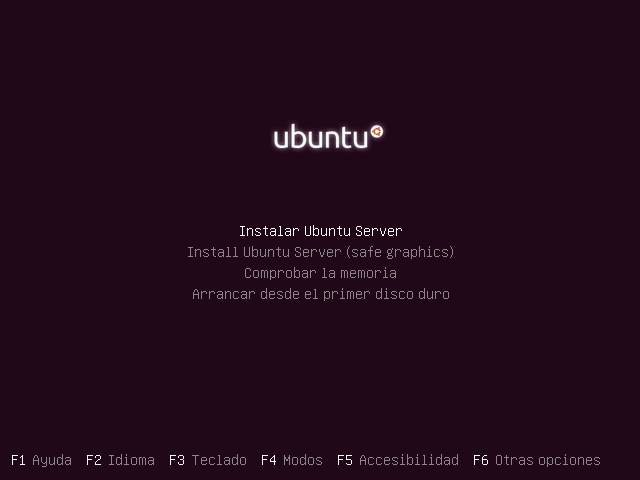
\includegraphics[width=15cm]{ubuntu_1.png}
    \vspace{-20pt}
\end{center}

A partir de aquí comenzará el instalador y los pasos que nos aparecerán serán los siguientes (algunos de estos pasos puede que no estén 100\% traducidos al castellano):

\begin{enumerate}
    \item Elegir el idioma del sistema
    \item Actualización del instalador:
    \begin{itemize}
        \item Si la máquina virtual se puede conectar a internet, comprobará si existe una actualización del propio instalador de Ubuntu.
        \item Podemos darle a “Continuar sin actualizar”
    \end{itemize}
    \item Configuración del idioma del teclado
    \item Configuración de la red
    \item Configuración del proxy de red
    \item Configuración del “mirror” o servidor espejo desde donde descargarse los \hyperlink{paquete_de_software}{paquetes de software} para las actualizaciones posteriores.
    \item Selección del disco duro donde realizar la instalación
    \item Elegir el particionado de disco.
    \item Configuración del perfil. Introduciremos el nombre de usuario, el nombre del servidor y la contraseña del usuario que vamos a crear.
    \item Configuración de SSH Server. Aceptaremos que se instale el servidor SSH durante la instalación. En caso de no seleccionar esta opción, posteriormente podremos realizar la instalación.
    \item “Featured Server Snaps”. En esta pantalla nos permite instalar software muy popular en servidores.
\end{enumerate}


Una vez le demos a continuar, comenzará la instalación en el disco duro. Debido a que durante la instalación tenemos conexión a internet, el propio instalador se descarga las últimas versiones de los paquetes de software desde los repositorios oficiales.


Al terminar la instalación, tendremos que reiniciar la máquina virtual.

\section{Post-instalación}
Tras realizar el reinicio de la máquina virtual nos encontraremos con que el sistema arranca en el sistema recién instalado, y que tendremos que loguearnos introduciendo el usuario y la contraseña utilizadas en la instalación.

\subsection{Actualización del sistema}
Por si acaso, realizaremos la actualización del índice del repositorio, actualizaremos el sistema y en caso necesario realizaremos un nuevo reinicio:

\begin{mycode}{Actualizar Ubuntu}{console}{}
mikeldi@ubuntu:~$ sudo su
[sudo] password for mikeldi:
root@ubuntu:~# apt update
...
root@ubuntu:~# apt upgrade
...
\end{mycode}

Con estos comandos nos aseguramos que el sistema está actualizado a los últimos paquetes que están en el repositorio.


\hypertarget{configurar_ip_estatica_ubuntu}{}
\subsection{Poner IP estática}
Debido a la configuración de red de nuestro servidor, la IP está puesta en modo dinámica, esto quiere decir que nuestro equipo ha cogido la IP por configuración de DHCP de nuestra red. Debido a que un servidor debe de tener IP estática, tenemos que realizar la modificación adecuada para ponerle la IP estática que mejor nos convenga. Para ello editaremos el fichero de configuración situado en la siguiente ruta: \configfile{ /etc/netplan/00-installer-config.yaml }

Lo modificaremos para que sea parecido a (siempre teniendo en cuenta la IP y gateway de nuestra red):


\begin{mycode}{Configurando IP estática en Ubuntu}{yaml}{}
network:
  ethernets:
    enp1s0:
      dhcp4: no
      addresses:
      - 192.168.200.10/24
      gateway4: 192.168.200.1
      nameservers:
        addresses: [8.8.8.8]
  version: 2
\end{mycode}

El fichero de configuración que hemos modificado es de tipo \href{https://es.wikipedia.org/wiki/YAML}{YAML}, que es un formato de texto que suele ser utilizado en programación o en ficheros de configuración. Este tipo de ficheros tiene en cuenta los espacios para el uso de la identación, y no suele permitir el uso de tabuladores.

Para aplicar los cambios realizados en el fichero de configuración deberemos ejecutar el siguiente comando que aplicará los cambios:

\begin{mycode}{Aplicar configuración de IP}{console}{}
root@ubuntu:~# netplan apply
\end{mycode}

\clearpage

\graphicspath{{../../../anexos/}}
\chapter{Glosario}

A continuación se expone un glosario de términos con sus correspondientes definiciones:

\begin{description}
    \hypertarget{altadisponibilidad}{}
    \item[Alta Disponibilidad:] Es un diseño de arquitectura de sistemas y la implementación que asegura que el servicio instalado y otorgado sea funcional sin que haya parada en el mismo. Esta arquitectura trata de que no haya ningún \hyperlink{spf}{\textit{single point of failure} (punto único de fallo)} en la misma.

    \hypertarget{cluster}{}
    \item[Clúster:] Se denomina clúster a un conjunto de ordenadores unidos entre sí mediante conectividad de red que actúan como si de un único servidor se tratara. Dependiendo del tipo de clúster que se va a crear, debe de ser pensado desde el diseño del servicio, ya que es la aplicación o servicio quién se encarga de crear el clúster (como ocurre con MySQL Cluster).

    \hypertarget{dependencia_software}{}
    \item [Dependencia de software:] Cuando se crea cualquier tipo de software lo habitual es hacer uso de otro software (librerías de seguridad, acceso a disco, codecs de vídeo, librerías 3D…) que son necesarias para el correcto funcionamiento de nuestro programa. Este otro software (que puede ser propio o ajeno) se denomina \textbf{dependencia}, ya que sin él, nuestro programa no funcionará y es necesario que exista en el sistema para hacer funciona nuestro programa.

    En las \hyperlink{distribucion_gnu_linux}{distribuciones GNU/Linux} se hace uso de los denominados \hyperlink{paquete_de_software}{paquetes de software} en los cuales se indican las dependencias que necesitan para funcionar y que por tanto se instalarán a la par que el programa elegido, por lo que nos aseguramos que el software instalado funcionará en cuanto termine la instalación.

    En caso de descargar un software ajeno de los \hyperlink{repositorio_de_software}{repositorios} oficiales de la distribución, es posible que necesitemos completar esas dependencias por nuestra cuenta, pero hoy en día es habitual que los creadores de software lo tengan en cuenta y esas dependencias estén en los repositorios oficiales.

    \hypertarget{distribucion_gnu_linux}{}
    \item [Distribución GNU/Linux:] Es una distribución de software basada en el núcleo Linux que incluye software \hyperlink{gnu}{GNU} para componer un Sistema Operativo que pueda ser utilizado por los usuarios. Cada distribución suele \hyperlink{paquete_de_software}{empaquetar el software} en un formato propio que aparte del propio software indica las \hyperlink{dependencia_de_software}{dependencias} de software que necesita para funcionar, por lo que hace que la instalación del software se realice de manera sencilla. El software de la distribución está almacenado en los \hyperlink{repositorio_de_software}{repositorios de software} oficiales de la distribución.

    Las distribuciones suelen estar orientadas para un uso generalizado, pero es cierto que algunas, por su historia o por su manera de entender el empaquetado de software, se necesitan más conocimientos, pero hoy en día no es lo habitual.

    Existen muchas distribuciones GNU/Linux, pero las que podríamos destacar son \hyperlink{ubuntu}{Ubuntu}, Debian, Red Hat y CentOS, que son las de mayor uso hoy en día a nivel profesional.

    \hypertarget{escalado_horizontal}{}
    \item[Escalado Horizontal:] Se llama escalado horizontal a la infraestructura que crece de manera horizontal añadiendo más servidores del mismo servicio. Estos servidores serán accesibles mediante un proxy o de manera directa, y todos contarán con el mismo servicio (web, base de datos, …). No confundir con un clúster, ya que la relación de los servidores en el escalado horizontal no tienen por qué ir en clúster.

    \hypertarget{escalado_vertical}{}
    \item[Escalado Vertical:] Es el incremento de hardware de un servidor. Supongamos que un servidor empieza a tener problemas de carga, pues con el escalado vertical se le añadiría más RAM, más procesador y/o discos duros más rápidos (en caso de ser una máquina virtual sería sencillo, en caso contrario habría que realizar la migración a un servidor nuevo).

    \hypertarget{gnu}{}
    \item[GNU:] Del acrónimo \textbf{GNU’s Not Unix} (GNU no es Unix) es un sistema operativo y un conjunto de programas libres cuyo origen surgió de la idea de crear un sistema operativo Unix basado en \hyperlink{software_libre}{Software Libre}.

    El desarrollo de GNU nació en 1983 por Richard Stallman comenzando por el compilador GCC, al que se fueron uniendo todo tipo de software y creando la Free Software Foundation (o FSF, fundación por el software libre) la cual creó la \hyperlink{licencias_libres}{licencia libre} más conocida actualmente: la \textbf{GPL} (GNU General Public License).

    El proyecto GNU avanzó en el tiempo y creó el kernel Hurd, pero bien es cierto que nunca llegó a ser funcional del todo y actualmente el kernel más utilizado es Linux, pero no es el único, ya que el software GNU también es usado en conjunto con otros kernels como son los \textbf{*BSD}, de ahí la importancia que cuando hacemos referencia al sistema operativo se haga uso de \hyperlink{gnu_linux}{GNU/Linux}.

    \hypertarget{gnu_linux}{}

    \itemimage{GNU/Linux:}{r}{0.21}
    {img/Gnulinux.svg.png}
    {\href{https://es.wikipedia.org/wiki/GNU/Linux\#/media/Archivo:Gnulinux.svg}{GNU/Linux: Wikipedia}}
    {
        Aunque comúnmente solemos llamar a las \hyperlink{distribucion_gnu_linux}{distribuciones} como “Linux” esto no suele ser correcto ya que en la distribución aparte del kernel va un conjunto enorme de software del proyecto GNU. Por lo tanto, lo ideal siempre es hacer uso del nombre completo GNU/Linux.

        El proyecto \hyperlink{gnu}{GNU} y sus herramientas y software son usados con otros kernels como son los *BSD en distribuciones como FreeBSD u OpenBSD. También existen versiones con kernel BSD para la distribución Debian, por lo que en ese caso sería “Debian GNU/BSD”.
    }


    \hypertarget{json}{}
    \item[JSON:] Es un formato de texto sencillo para el intercambio de datos. Aunque originalmente fue creado como notación de objetos para Javascript, su amplia utilización ha hecho que sea utilizado como alternativa a XML.


    \hypertarget{licencias_libres}{}
    \item[Licencias libres:] Una licencia de software es un contrato entre el creador (o el titular de los derechos de autor) del software y el usuario. Todo software que usamos suele exigir la lectura de esta licencia y es por ello muy importante conocer qué se puede y no se puede hacer con dicho software.

    Las licencias libres son aquellas que nos permiten hacer con el software lo que las cuatro libertades del \hyperlink{software_libre}{Software Libre} exige.

    Entre las licencias libres más utilizadas hoy en día están la GPL (General Public License del proyecto \hyperlink{gnu}{GNU}), la Apache License, algunas de las versiones de las licencias Creative Commons, …


    \hypertarget{linux}{}
    \item[Linux:] Creado originalmente por Linus Torvalds en 1991 y actualmente desarrollado por cientos de desarrolladores de todo el mundo, Linux es el núcleo (o kernel) gratuito y libre similar al núcleo de los sistemas operativos Unix.

    Comenzó como un proyecto personal de Linus (siendo estudiante universitario) para su ordenador 386 y actualmente está portado a \href{https://es.wikipedia.org/wiki/Portabilidad\_del\_n\%C3\%BAcleo\_Linux\_y\_arquitecturas\_soportadas}{decenas de plataformas hardware}. Es el proyecto más grande y ambicioso del \hyperlink{software_libre}{Software Libre}, aunque originalmente no se permitía el uso comercial del mismo (hasta la versión 0.12).

    Al poco tiempo de comenzar su desarrollo el proyecto \hyperlink{gnu}{GNU} lo adoptó como su kernel naciendo lo que actualmente conocemos como \hyperlink{gnu_linux}{GNU/Linux} y con ello cientos de \hyperlink{distribucion_gnu_linux}{distribuciones}.

    Es un núcleo de tipo monolítico que permite la carga de módulos en tiempo de ejecución


    \hypertarget{lts}{}
    \item[LTS:] Del inglés \textit{\textbf{L}ong \textbf{T}erm \textbf{S}upport} (en castellano “soporte a largo plazo”), es una característica en informática que hace referencia a versiones especiales de software que contarán con un soporte más largo del habitual, por lo que serán las versiones idóneas para usar en servidores.

    Estas versiones suelen contar con actualizaciones de seguridad, pero no con cambios notorios en la forma del software para fomentar la fiabilidad del mismo. Lo habitual es utilizar este tipo de versiones en servidores, que aunque puedan no tener las últimas modificaciones de las versiones más recientes del software, nos aseguramos la fiabilidad. Esto hace que tengamos que decidir si es necesario contar con las características de las últimas versiones (ya sea nuevos servicios, opciones nuevas, velocidad, … ) o si preferimos contar con una versión que tendrá un ciclo de vida más longevo pero con actualizaciones de seguridad.

    Es habitual verlo en proyectos de \hyperlink{software_libre}{Software Libre}, como ejemplos podemos tomar el kernel \hyperlink{linux}{Linux} (actualmente la versión 5.4.58 es la denominada LTS) y la distribución \hyperlink{ubuntu}{Ubuntu} (en este caso la versión 20.04).


    \hypertarget{paquete_de_software}{}
    \item[Paquetes de Software:] Un paquete de software no es más que una manera de poder distribuir el software creado. En \hyperlink{distribucion_gnu_linux}{distribuciones GNU/Linux} estos paquetes determinan las \hyperlink{dependencia_software}{dependencias} que necesitan para que su instalación sea lo más sencilla posible.

    Lo habitual es que estos paquetes estén gestionados mediante un sistema de gestión propio para conocer cuáles están instalados, sus dependencias, desinstalarlos de manera sencila...

    No sólo se usa en distribuciones GNU/Linux, ya que varios lenguajes de programación hacen lo propio para distribuir software en forma de paquetes. Como ejemplos:
    \begin{itemize}
        \item En distribuciones GNU/Linux tenemos APT, Yum, Zypper, Portage, ...
        \item En lenguajes de programación tenemos Gem para Ruby, Eggs para Python, CPAN en Perl, ...
    \end{itemize}


    \hypertarget{repositorio_de_software}{}
    \item[Repositorio de Software:] Se podría denominar repositorio como el almacén donde se guardan los \hyperlink{paquete_de_software}{paquetes de software}. Las \hyperlink{distribucion_gnu_linux}{distribuciones GNU/Linux} cuentan con sus repositorios oficiales, donde se almacena el software para cada versión que tiene la distribución.

    Aparte del software que podemos instalar, también cuentan con un índice para saber los paquetes y las versiones que se almacena en ellos. Este índice es necesario que lo actualicemos de manera periódica (en Ubuntu ejecutando: “apt update”) ya que gracias a él sabremos si tenemos que realizar actualizaciones de los paquetes instalados.

    También podemos utilizar repositorios externos al de la distribución, repositorios oficiales de un software por ejemplo, que nos permiten instalar la última versión de ese software sobre nuestra distribución. Cuando un paquete con el mismo nombre existe en distintos repositorios, siempre se instalará del repositorio que tenga la versión más nueva.

    No es buena práctica, y \textbf{está completamente desaconsejado}, mezclar repositorios de distribuciones distintas aunque el gestor de paquetes sea el mismo (usar repositorios de Debian en Ubuntu o viceversa).


    \hypertarget{spf}{}
    \item[Single Point of Failure:] O punto único de fallo, es un componente de un sistema que tras un fallo en su funcionamiento ocasiona un fallo global en el sistema completo, dejándolo inoperante. Un SPOF puede ser un componente de hardware, software o eléctrico.


    \hypertarget{software_libre}{}
    \item[Software Libre:] El movimiento del Software Libre fue creado por Richard Stallman a la par que creaba el proyecto \hyperlink{gnu}{GNU}. Para que un software sea considerado como Software Libre debe contener una \hyperlink{licencias_libres}{licencia libre} que debe otorgar las cuatro libertades siguientes:
    \begin{itemize}
        \item Libertad de usar el software para cualquier propósito.
        \item Libertad de estudiar el software y su funcionamiento interno (es por ello necesario poder acceder al código fuente).
        \item Libertad de distribuir el software con quien queramos.
        \item Libertad de poder modificar y mejorar el software según nos interese.
    \end{itemize}

    Es muy importante tener en cuenta que Software Libre no significa gratis, ya que en inglés el término viene de Free Software donde “Free” puede significar libre y gratis. Es cierto que la gran mayoría del Software Libre puede ser gratis, pero no todo el software gratis es Software Libre.


    \hypertarget{ssh_server}{}
    \item [SSH Server]: De \textbf{S}ecure \textbf{SH}ell, es el nombre de un protocolo y del programa (tanto servidor, como cliente) cuya función principal es la de acceder de manera remota a través de un canal seguro a un servidor.

    SSH permite no sólo la conexión a un servidor sino también la transferencia de ficheros y creación de túneles cifrados por los que pueden viajar otros protocolos. El puerto habitual de uso para este protocolo es el \textbf{22}.


    \hypertarget{systemd}{}
    \item [Systemd]: es un conjunto de demonios de administración de sistema, bibliotecas y herramientas diseñados como una plataforma de administración y configuración central para interactuar con el núcleo del Sistema operativo \hyperlink{gnu_linux}{GNU/Linux}.


    \hypertarget{ubuntu}{}

    \itemimage{Ubuntu:}{r}{0.21}
    {img/ubuntu.svg.png}
    {\href{https://es.wikipedia.org/wiki/Ubuntu}{Ubuntu: Wikipedia}}
    {
        Es una \hyperlink{distribucion_gnu_linux}{distribución de GNU/Linux} originalmente basada en Debian y creada por la compañía Canonical en el 2004. En su momento fue una de las distribuciones que apostaron por un sistema de instalación sencillo y con la intención de detectar el máximo hardware posible para acercarse a la gran cantidad de usuarios posibles.

        Hoy en día es una de las distribuciones más utilizadas tanto a nivel de escritorio como a nivel de servidores ya que cuenta con dos versiones separadas a la hora de realizar la instalación (aunque realmente es la misma distribución).

        Una de sus ventajas es la creación de versiones \hyperlink{lts}{LTS} cada dos años, que son versiones que garantizan su soporte técnico durante más tiempo por lo que supone una ventaja a la hora de realizar la instalación en servidores. Con ellos nos aseguramos que el software va a ser actualizado ante fallos de seguridad durante más tiempo que las versiones que no son LTS.
    }


\end{description}

\clearpage

\end{document}
